\section{Optimal Room Traversal with Macro-Edges}

After interior nodes are eliminated, macro-edges between selected pairs of
perimeter nodes have to be added to ensure that rectangles can be traversed
optimally.  A straightforward approach would be adding a macro-edge between any
two nodes on the perimeter of a rectangle
This strategy is optimal but has the disadvantage of creating a branching 
factor quadratic in the number of perimeter nodes. 
We introduce an alternative strategy, that creates much fewer
macro-edges, by defining a \emph{dominance} relation between macro-edges.

\begin{definition}
\label{def:dominance}
A macro-edge connecting two arbitrary nodes $t_1$ and $t_2$ in a perimeter
clique is non-dominated if all other paths between $t_1$ and $t_2$ in the
perimeter clique have a cost strictly larger than the macro-edge at hand.
\end{definition}

There are three cases to discuss. In each case the length of each added macro-edge 
is equal to the heuristic distance between its two endpoints -- as measured
using Octile distance.
\par \noindent
\textbf{Case 1:} nodes on the same side of the perimeter. These are connected
just as in the original grid.
\par \noindent
\textbf{Case 2:} nodes on orthogonal sides of the perimeter.
These are connected \emph{iff} the shortest path between them is a diagonal
(45-degree) line; this is illustrated in Figure \ref{fig-macroedges} (Left).
\par \noindent
\textbf{Case 3:} nodes on opposite sides of the perimeter. For each such node we
generate a ``fan'' of neighbours from the opposite side.  
Figure \ref{fig-macroedges} (Right), illustrates
this idea.  Starting from a node such as $t_{1}$ we step to the closest
neighbour from the opposite side of the rectangle and extend the fan by progressing away
from the middle in both directions adding each node we encounter.  The last node
on either side of the fan is placed diagonally, at 45 degrees, from $t_{1}$
(such as $t_{2}$) or located in the corner of the perimeter (whichever we
encounter first).  There is no need to add further nodes, such as $t_{3}$, as
these can be reached optimally from $t_1$ via the path $< t_1, t_2, \dots,
t_3 > $.

\par
Using Definition \ref{def:dominance} it is easy to see that each edge we compute
is non dominated. Further, all non-dominated edges are necessary to ensure
optimality. 

\begin{lemma} \label{lemma-rooms} Let $R$ be an empty rectangle in
an 8-connected grid map. Let $m$ and $n$ be two perimeter locations.
Then, $m$ and $n$ can be connected optimally through a path that
contains only non-dominated macro-edges.
\end{lemma}

\begin{proof}:
We split the proof over the 3 cases discussed earlier.
In the first case we walk along the perimeter from $m$ to $n$; the
optimality of this path is immediate. In the second and third case 
the two nodes can be connected through an optimal path that has one diagonal macro-edge
(at one end of the path) and zero or more straight macro-edges.
See again the example of travelling from $t_1$ to $t_3$ in Figure
\ref{fig-macroedges} (Right).
\end{proof}

\begin{figure}[tb]
       \begin{center}
		   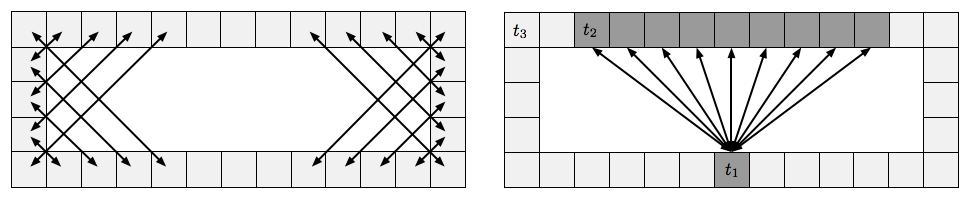
\includegraphics[width=0.97\columnwidth, trim = 10mm 10mm 10mm 0mm]
			{diagrams/macroedges_wide.png}
       \end{center}
	\vspace{-3pt}
       \caption{(Top) Macro edges between nodes on orthogonal sides of an empty
       rectangle. (Bottom) Each node on the perimeter is connected to a set of 
		nodes on the opposite side.}
       \label{fig-macroedges}
\end{figure}

\noindent
\textbf{Node Insertion:}
When the start or goal is a node from the interior of an empty rectangle we
will use a procedure that temporarily re-inserts nodes back into the 
graph for the duration of a search.
{If the start and goal are interior nodes
in the same room no insertion is necessary; an optimal path is trivially
available. } {Otherwise, we add four ``fans'' (collections) of macro edges.  Each fan connects
the start (goal) node to a set of nodes on one side of the rectangle's
perimeter.  Fans are built as shown earlier.}
To prove optimality is retained we run the argument given
for Case 3 of Lemma \ref{lemma-rooms}, substituting $m$ for the newly inserted node.
\par
Given the simple geometry of rectangles, it is possible to identify in constant
time the set of nodes which the start or goal must be connected to.  Further,
these neighbours could be generated on-the-fly.

%We claim that using the temporary macro edges added by this algorithm it is possible to travel optimally from the start or goal 
%location to any node on the perimeter of the start or goal rectangle. 
%\par \noindent
%\newline
\begin{theorem}
For every optimal path $\pi$ on an original grid, there exists an optimal path
$\pi'$ on the modified graph with the property that $\pi$ and $\pi'$ have the
same cost.
\end{theorem}
\begin{proof}
Consider an optimal path $\pi$ on the original map and a rectangle $R$ that is
crossed by $\pi$.  Let $m$ and $n$ be the two perimeter points along $\pi$.
According to Lemma~\ref{lemma-rooms}, there is a way to connect $m$ and $n$
optimally in the modified graph. Thus, we can replace the original segment $[m
\dots n]$ in $\pi$ with the cost-wise equivalent segment that corresponds to the
modified graph.  The case when $m$ (or $n$) is the start or goal node is
addressed similarly.  By performing such a
path segment replacement for all rectangles intersected by $\pi$, we obtain a
path $\pi'$ that satisfies the desired properties.
\end{proof}

%\textbf{Optimality:} We claim the symmetry elimination procedure outlined in this section is sufficient to guarantee
%that A*, running on a modified 8-connected grid map, will always find an optimal length solution if one exists.
%Our argument follows from Lemma \ref{lemma-rooms} and Lemma \ref{lemma-insertion}.
%It is based on the observation that for every segment of an optimal length path, which enters a rectangle at some node $m$,
%traverses through the interior of the rectangle and exits at some node $n$, there is an equivalent length path that mentions only 
%nodes from the perimeter of that rectangle and possibly one macro edge.

